\documentclass[11pt, oneside]{article} 
\usepackage{geometry}
\geometry{letterpaper} 
\usepackage{graphicx}
	
\usepackage{amssymb}
\usepackage{amsmath}
\usepackage{parskip}
\usepackage{color}
\usepackage{hyperref}

\graphicspath{{/Users/telliott/Github/calculus_book/png/}}
% \begin{center} 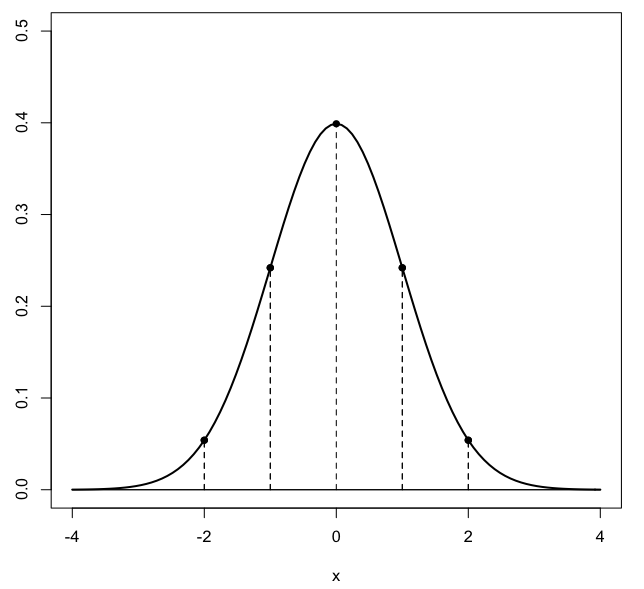
\includegraphics [scale=0.4] {gauss3.png} \end{center}

\title{Sum of cubes}
\date{}

\begin{document}
\maketitle
\Large

\label{sec:sum_of_cubers}

The formula is
\[ \sum\limits_{k=1}^n k^3 = [ \ \sum\limits_{k=1}^n k \ ] ^2 \]

\begin{center} 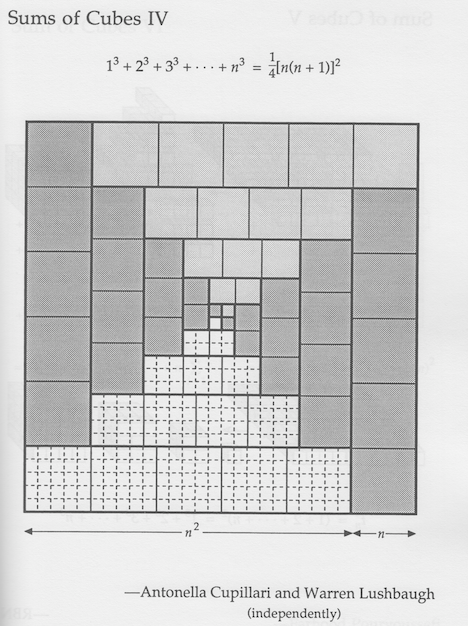
\includegraphics [scale=0.4] {sum_n3.png} \end{center}

Let's prove this using induction.

The "base case" is pretty simple.  For $n=2$
\[ 1^3 + 2^3 = 1 + 8 = 9 \]
and
\[ \frac{n^2(n+1)^2}{2^2} = \frac{2^2(3^2)}{2^2} = 3^2 = 9 \]

Now for the induction step what we need to show is that what we get assuming the formula for $n$ is correct and then adding the term $(n+1)^3$

\[ \frac{n^2(n+1)^2}{2^2} + (n+1)^3 \]
is equal to what we get by plugging $n+1$ into the formula.
\[ \frac{(n+1)^2(n+2)^2}{2^2} \]

We need to show that eqn 2 is equal to eqn 3.  
\[ \frac{n^2(n+1)^2}{2^2} + (n+1)^3 = \frac{(n+1)^2(n+2)^2}{2^2} \]

First, we can factor out and cancel $(n+1)^2$ from both sides.  So then we have
\[ \frac{n^2}{2^2} + (n+1) \stackrel{?}{=} \frac{(n+2)^2}{2^2} \]
\[ n^2 + 4(n+1) \stackrel{?}{=} (n+2)^2 \]
That looks correct!

$\square$

\subsection*{derivation by collapsing sum}

We proceed exactly as before
\[ (k+1)^4 = k^4 + 4k^3 + 6k^2 + 4k + 1 \]

Sum each term from $k=1 \rightarrow k=n$

\[ \sum_{k=1}^n (k+1)^4 = \sum_{k=1}^n k^4 + \sum_{k=1}^n 4k^3 + \sum_{k=1}^n 6k^2 + \sum_{k=1}^n 4k + \sum_{k=1}^n 1 \]

Rearrange and compute the collapsing sum.

\[ \sum_{k=1}^n (k+1)^4 - \sum_{k=1}^n k^4 = \sum_{k=1}^n 4k^3 + \sum_{k=1}^n 6k^2 + \sum_{k=1}^n 4k + \sum_{k=1}^n 1 \]

\[ (n+1)^4 - 1 = \sum_{k=1}^n 4k^3 + \sum_{k=1}^n 6k^2 + \sum_{k=1}^n 4k + \sum_{k=1}^n 1 \]

Substitute for the right-hand sum

\[ (n+1)^4 - 1 = \sum_{k=1}^n 4k^3 + \sum_{k=1}^n 6k^2 + \sum_{k=1}^n 4k + n \]

Rearrange some more

\[ \sum_{k=1}^n 4k^3 = (n+1)^4 - 1 - \sum_{k=1}^n 6k^2 - \sum_{k=1}^n 4k - n \]

Expand the term $(n+1)^4$ and pick up the $-1 - n$:

\[ (n+1)^4 - 1 - n \]
\[ = n^4 + 4n^3 + 6n^2 + 4n + 1 - 1 - n \]
\[ =  n^4 + 4n^3 + 6n^2 + 3n  \]

Factor out an $n$

\[ = (n)(n^3 + 4n^2 + 6n + 3) \]

And another $n+1$

\[ = (n)(n+1)(n^2 + 3n + 3) \]

Recall our previous results:

\[ \sum_{k=1}^n 6k^2 = 6 \sum_{k=1}^n k^2 \]
\[ = 6 \ \frac{n(n+1)(2n+1)}{6}  \] 
\[ = n(n+1)(2n+1) \] 

Similarly

\[ \sum_{k=1}^n 4k = 4 \sum_{k=1}^n k \]
\[ = 4 \ \frac{n(n+1)}{2} \]
\[ = 2 n(n+1) \]

Substitute all three of these results (and pull out the factor of $4$ from the sum):

\[ 4\sum_{k=1}^n k^3 = (n)(n+1)(n^2 + 3n + 3) - n(n+1)(2n+1) -  2 n(n+1) \] 

Just a bit more algebra.  See that we have $n(n+1)$ in each term.  We have

\[ = n(n+1) \ [ \ (n^2 + 3n + 3) - (2n+1) -  2 \ ]  \]
\[ = n(n+1) \ [ \ n^2 + 3n + 3 - 2n - 1 -  2 \ ]  \]
\[ = n(n+1) \ [ \ n^2 + n  \ ]  \]
\[ = n(n+1)  \cdot  n(n+1)  \]

So all together we have

\[ 4\sum_{k=1}^n k^3 = n(n+1) \cdot n (n+1) \] 
\[ \sum_{k=1}^n k^3 = \frac{n(n+1)}{2} \cdot \frac{n (n+1)}{2} \] 
\[ \sum_{k=1}^n k^3 = \ [ \ \frac{n(n+1)}{2} \ ]^2 \] 
A remarkable simplification! 

\subsection*{Looking deeper}

\[ \sum\limits_{k=1}^n k^3 = [\ \sum\limits_{k=1}^n k \ ] ^2 \]
We want to try to understand something more about why this is true.  

A web search revealed the answer.  Here's an interesting pattern for the cubes of integers
\[ 1^3 = 1 \]
\[ 2^3 = 8 = 3 + 5 \]
\[ 3^3 = 27 = 7 + 9 + 11 \]
\[ 4^3 = 64 = 13 + 15 + 17 + 19 \]
\[ 5^3 = 125 = 21 + 23 + 25 + 27 + 29  \]

If you want a formula for $n^3$, notice that the first term is $n^2 - n + 1$ and the last term is $n^2 - n + 2n - 1$, and the number of terms for each sum equals $n$.  (There are $n$ odd numbers between $1$ and $2n-1$).

In other words, the sum of all the cubes of integers from $1^3$ to $n^3$ is equal to the sum of all the odd numbers up to $n^2 - n + 2n - 1 = n^2 + n - 1$.

How many of these numbers are there?  A little thought should convince you that the answer is $(n^2 + n)/2$.  For example, with $n=5$, our last odd number is $5^2 + 5 - 1 = 29$, and we have $(25 + 5)/2 = 15$ terms.

We want the sum of the first $(n^2 + n)/2$ odd numbers.

Let's look at another pattern
\[ 1 = 1 \]
\[ 2^2 = 4 = 1 + 3 \]
\[ 3^2 = 9 = 1 + 3 + 5 \]
\[ 4^2 = 16 = 1 + 3 + 5 + 7 \]
\[ 5^2 = 25 = 1 + 3 + 5 + 7 + 9 \]

The \emph{odd number theorem} says that the sum of the first $n$ odd numbers is equal to $n^2$.  We want the sum of the first $(n^2 + n)/2$ odd numbers, so that's $((n^2 + n)/2)^2$.  And that's how we get our formula.

Here is another beautiful proof without words:

\begin{center} 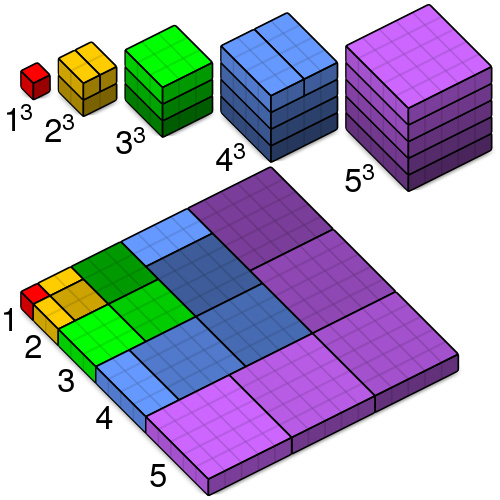
\includegraphics [scale=0.4] {sum_cubes.png} \end{center}

The length of the bottom pattern is a triangular number, which is itself a sum of squares.  When squared it equals the sum of cubes.

\subsection*{another method}
Here is another approach that I found very early in Hamming (Chapter 2) and have not seen in other books.  It is called the method of \emph{undetermined coefficients}.  

We observe that the sum of integers formula has order $n^2$, while the sum of squares has order $n^3$, so we expect the sum of cubes would have $n^4$.

\[ \sum_{k=0}^{k=n} k^3 = an^4 + bn^3 + cn^2 + dn + e \]
and if $n=0$ the sum is zero so $e = 0$.

The right-hand side is 
\[ an^4 + bn^3 + cn^2 + dn \]

The inductive step is to write the formula for $m-1$, and then add $m^3$ to it.

The right-hand side is just the formula, writing $m$ for $n$
\[ am^4 + bm^3 + cm^2 + dm \]

The left-hand side is the formula for $(m-1)$, plus $m^3$ from the induction step:
\[ a(m-1)^4 + b(m-1)^3 + c(m-1)^2 + d(m-1) + m^3 \]

We work with the left-hand side.  Expand each term using the binomial theorem:
\[ a \ [ \ m^4 - 4m^3 + 6m^2 - 4m + 1 \ ]  \]
\[ b \ [ \ m^3 - 3m^2 + 3m -1 \ ]  \]
\[ c \ [ \ m^2 - 2m + 1 \ ]  \]
\[ d \ [ \ m - 1 \ ]  \] 

Next, group the cofactors by the corresponding powers:
\[  \ [ \ a \ ] \ m^4 \]
\[  \ [ \ -4a + b + 1 \ ] \ m^3 \]
\[  \ [ \ 6a - 3b + c \ ] \ m^2 \]
\[  \ [ \ -4a + 3b - 2c + d \ ] \ m \]
\[ a - b + c - d \]
Now to the point.  The cofactors for \emph{each power} of $m$ must cancel exactly.

$am^4$ cancels on left and right, likewise $bm^3$, $cm^2$ and $dm$.  That leaves four equations.
\[ -4a + 1 = 0 \]
\[ 6a - 3b = 0 \]
\[ -4a + 3b - 2c = 0 \]
\[ a - b + c - d = 0 \]

We find that $a = 1/4$, $b = 1/2$, $c = 1/4$, $d = 0$.  So then finally the formula is
\[ an^4 + bn^3 + cn^2 + dn \]
\[ = \frac{n^4 + 2n^3 + n^2}{4} \]
\[ \frac{(n^2 + n)^2}{2^2} = \ [ \ \frac{n(n+1)}{2} \ ]^2 \]
which is exactly what we will have from other approaches.

Hamming uses this method to get a general formula, but we will not need that, because we will show how to use the binomial theorem to get what is necessary.


\end{document}  